% ------------------------------------------------------------------------------
% TYPO3 Version 10.3 - What's New (Dutch Version)
%
% @license	Creative Commons BY-NC-SA 3.0
% @link		https://typo3.org/help/documentation/whats-new/
% @language	Dutch
% ------------------------------------------------------------------------------

\section{Beveiliging en privacy}
\begin{frame}[fragile]
	\frametitle{Beveiliging en privacy}

	\begin{center}\huge{Hoofdstuk 5:}\end{center}
	\begin{center}\huge{\color{typo3darkgrey}\textbf{Beveiliging en privacy}}\end{center}

\end{frame}

% ------------------------------------------------------------------------------
% Feature | 90333 | Dashboard

\begin{frame}[fragile]
	\frametitle{Beveiliging en privacy}
	\framesubtitle{Dashboard}

	\begin{itemize}
		\item Widgets op Dashboards kunnen gevoelige informatie bevatten.
		\item Daarom wordt aangeraden om toegangspermissies voor widgets op basis van een groep in te stellen.
		\item Backendgebruikers kunnen alleen bij widgets die voor hen beschikbaar zijn.
		\item Gebruikers met adminrechten hebben altijd toegang tot alle widgets.
	\end{itemize}

\end{frame}

% ------------------------------------------------------------------------------
% Feature | 89978 | Introduce Status Report for insecure exception handler settings

\begin{frame}[fragile]
	\frametitle{Beveiliging en privacy}
	\framesubtitle{Statusrapportages}

	\begin{itemize}
		\item De DebugExceptionHandler kan mogelijk gevoelige data uitvoeren dat kan
			resulteren in een kwetsbaarheid die informatie ontsluit.
		\item Een nieuwe statusrapportage waarschuwt admins hiervoor.
	\end{itemize}

	\vspace{0.4cm}
	\textbf{WAARSCHUWING}, als context \textbf{development} is en foutmeldingen zijn ingeschakeld:
	\begin{figure}
		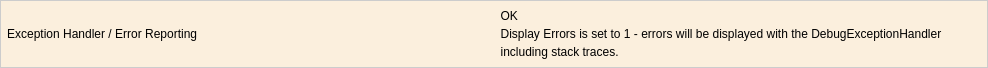
\includegraphics[width=1\linewidth]{SecurityAndPrivacy/89978a-IntroduceStatusReportForInsecureExceptionHandlerSettings.png}
	\end{figure}

	\textbf{FOUT}, als context \textbf{production} is en foutmeldingen zijn ingeschakeld:
	\begin{figure}
		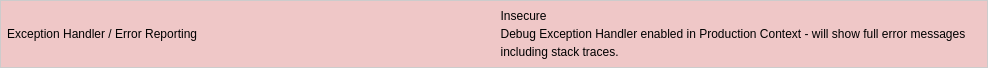
\includegraphics[width=1\linewidth]{SecurityAndPrivacy/89978b-IntroduceStatusReportForInsecureExceptionHandlerSettings.png}
	\end{figure}

\end{frame}

% ------------------------------------------------------------------------------
% Feature | 90351 | Allow TYPO3 to make SameSite cookies configurable

\begin{frame}[fragile]
	\frametitle{Beveiliging en privacy}
	\framesubtitle{SameSite Cookies (1)}

	\begin{itemize}
		\item Om beveiliging en privacy te verbeteren ondersteunt TYPO3 de "SameSite"-optie
			voor cookies van TYPO3.
		\item De attribuut wordt ondersteund door de meeste moderne browsers en laat websites
			aangeven als cookies beperkt moeten worden.
		\item Volgens:
			\href{https://www.owasp.org/index.php/SameSite}{OWASP}, zullen SameSite cookies\newline
			\small
				"\textit{het risico op cross-origin informatielekken tegengaan}", with\newline
				"\textit{enige bescherming bieden tegen cross-site request forgery aanvallen}".
			\normalsize

		\item Geldige waarden zijn "\textbf{strict}", "\textbf{lax}", of \textit{not set}.
	\end{itemize}

\end{frame}

% ------------------------------------------------------------------------------
% Feature | 90351 | Allow TYPO3 to make SameSite cookies configurable

\begin{frame}[fragile]
	\frametitle{Beveiliging en privacy}
	\framesubtitle{SameSite Cookies (2)}

	\begin{itemize}
		\item TYPO3 stelt de volgende opties in:

			\begin{itemize}\small
				\item FE gebruikerssessies: "lax" als standaard
				\item BE gebruikerssessies: "strict" als standaard
				\item Install Tool sessies: "strict" (niet instelbaar)
				\item Laatste aanmeldingsprovider (BE): "strict" (niet instelbaar)
			\end{itemize}\normalsize

		\item De Install Tool biedt systeemconfiguratie om de instellingen voor
			SameSite cookies aan te passen als de standaardinstellingen te strikt zijn
			(bijv. met authenticatieproviders zoals OpenID/OAuth).

		\item Voor meer informatie over SameSite cookies:
			\href{https://tools.ietf.org/html/draft-ietf-httpbis-cookie-same-site-00}{RFC6265} (draft).
	\end{itemize}

\end{frame}

% ------------------------------------------------------------------------------
% Feature | 90262 | Add Argon2id to password hash algorithms

\begin{frame}[fragile]
	\frametitle{Beveiliging en privacy}
	\framesubtitle{Wachtwoord Hash-algoritmes}

	\begin{itemize}
		\item Het hash-algoritme \texttt{Argon2i} ("i") werd toegevoegd in TYPO3 v9 LTS.
		\item \texttt{Argon2id} ("id") is nu ook beschikbaar in TYPO3 als de PHP-versie het ondersteunt.
		\item \texttt{Argon2id} is een hybride van \texttt{Argon2i} en \texttt{Argon2d}
			en is beter bestand tegen zijkanaal-aanvallen.
		\item \texttt{Argon2id} is meestal beschikbaar op systemen met PHP versie 7.3 of hoger.
	\end{itemize}

\end{frame}

% ------------------------------------------------------------------------------
